\documentclass[11pt,letterpaper]{article}
\PassOptionsToPackage{hyphens}{url}
\usepackage[margin=.83in,top=.8in,bottom=.8in,headheight=15pt]{geometry}
\usepackage[T1]{fontenc}
\usepackage{lmodern,amsmath,amssymb,mathtools,bm,booktabs,array,graphicx,tikz}
\usetikzlibrary{arrows.meta,positioning,calc,decorations.pathreplacing,patterns}
\definecolor{ink}{HTML}{17344D}\definecolor{accent}{HTML}{087E8B}\definecolor{pale}{HTML}{EDF5F5}\definecolor{gold}{HTML}{AD6B19}
\providecommand{\dd}{\,\mathrm{d}}\providecommand{\R}{\mathbb{R}}
\providecommand{\E}{\mathbb{E}}\providecommand{\Var}{\operatorname{Var}}
\providecommand{\Cov}{\operatorname{Cov}}\providecommand{\diag}{\operatorname{diag}}
\providecommand{\norm}[1]{\left\lVert#1\right\rVert}
\providecommand{\abs}[1]{\left|#1\right|}
\usepackage{microtype,hyperref,fancyhdr,enumitem,amsthm,sectsty,needspace}
\allsectionsfont{\raggedright}
\hypersetup{colorlinks=true,linkcolor=ink,urlcolor=accent,pdfauthor={Zan Ahmad},pdftitle={Surrogate error, amortized cost and training-step bias / Lecture notes}}
\setlength{\parindent}{0pt}\setlength{\parskip}{6pt}\linespread{1.07}
\setlist{itemsep=3pt,topsep=4pt,leftmargin=*}
\emergencystretch=2em\clubpenalty=10000\widowpenalty=10000
\pagestyle{fancy}\fancyhf{}\fancyhead[L]{\small Computational Cardiology}\fancyhead[R]{\small Lecture 19}
\fancyfoot[L]{\footnotesize Zan Ahmad}\fancyfoot[R]{\footnotesize\thepage}\renewcommand{\headrulewidth}{.3pt}
\newtheorem{proposition}{Proposition}\newtheorem{theorem}{Theorem}\newtheorem{lemma}{Lemma}
\theoremstyle{definition}\newtheorem{definition}{Definition}\newtheorem{example}{Example}
\numberwithin{equation}{section}
\begin{document}
{\small\scshape Computational Cardiology\hfill Lecture 19}\par\medskip
{\raggedright\hyphenpenalty=10000\exhyphenpenalty=10000\LARGE\bfseries\color{ink} Surrogate error, amortized cost and training-step bias\par}\medskip
{\small Lecture notes}\par\bigskip
A surrogate can be inexpensive per query while remaining inaccurate or expensive to prepare. Error and total cost therefore need separate definitions. A scalar decay problem then shows a subtler failure: refining the inference solver can converge more accurately to a generator that was biased by its training discretization.

\section{Reference error and approximation error}
\hypertarget{note-reference-error-and-approximation-error}{}\label{note:reference-error-and-approximation-error}
{\small \href{slides.html\#frame=three-solutions-in-an-error-budget\&step=1}{Slides for this section}}\par
A useful research claim specifies a task, a regime and an acceptable error. For example, a surrogate might approximate a fixed-time field over a stated family of initial conditions while using less total computation after a specified number of queries. Each phrase creates an obligation: define the field and time, identify the input family, choose an error metric, measure costs and test the query range. A vague claim that a method is fast and accurate cannot be disproved by a clear experiment.

There are at least three distinct comparisons. Surrogate error measures disagreement with a reference calculation. Numerical verification asks how closely that reference solves the intended equations. Biological validation asks whether those equations and parameters describe relevant measurements for the intended purpose. Agreement with a numerical reference can establish the first comparison while leaving the other two unresolved. Calling the reference ground truth in a data file does not eliminate its discretization error or modeling assumptions.

Our heat benchmark has an analytic solution, allowing numerical and surrogate errors to be measured separately. There are no biological observations in the fixture. The comparison therefore supports a computational claim only. Its value is the structure of the evidence, which can later be applied to a harder cardiac question with appropriate geometry, parameters and measurements.

\[
\|u_{\rm sur}-u\|\le\|u_{\rm sur}-u_{\rm ref}\|+\|u_{\rm ref}-u\|
\]
Use the same absolute norm and compatible fields. This triangle bound does not quantify error against biological reality.

Let $u$ be the solution of the stated differential equation, $u_{ref}$ a computed reference and $u_{sur}$ a surrogate output. The triangle inequality gives an error budget only when all three objects are compared in compatible coordinates, at the same time and in the same norm. It does not include discrepancy between the differential equation and a biological system.
\Needspace{10\baselineskip}
\section{Amortized computational cost}
\hypertarget{note-amortized-computational-cost}{}\label{note:amortized-computational-cost}
{\small \href{slides.html\#frame=total-reference-cost\&step=1}{Slides for this section}}\par
A trained method has setup costs. Depending on the workflow, these may include reference-data generation, preprocessing, graph construction, eigendecomposition, training, model selection and loading. Some costs are paid once for a model; others recur for each new geometry or parameter field. A per-query timing that excludes all of them answers a narrower question than total workflow cost. In the GFuNK context, the paper explicitly separates the spectral representation built for each geometry and diffusion setting from subsequent inference.

For a simple accounting model, let setup cost be C0, reference query cost Cr and surrogate query cost Cs. After Q queries, the reference costs QCr and the surrogate costs C0+QCs. If Cs is less than Cr, the surrogate becomes cheaper only after Q exceeds C0 divided by Cr\ensuremath{-}Cs. If Cs is not smaller, there is no positive amortization threshold under this model. The inequality must also satisfy the error requirement: a cheaper but scientifically inadequate result is not an acceptable replacement.

Our companion measures analytic-label generation and fitting separately from warm queries. The labels are deliberately cheap, since their closed form is known. This can produce a very small arithmetic break-even count, but that is not evidence for learning in real electrophysiology. The analytic spectral solution is included as a competing baseline because the best comparator for this transparent problem is not necessarily a general time-stepping solver.

\[
C_{\rm ref}(Q)=QC_r,\quad C_{\rm sur}(Q)=C_0+QC_s,\quad Q>\frac{C_0}{C_r-C_s}
\]
The last inequality applies only when Cr>Cs and both methods meet the stated error criterion.

With $C_r>C_s$, the first strictly cheaper integer query count is
\[
 Q_{min}=\left\lfloor\frac{C_0}{C_r-C_s}\right\rfloor+1.
\]
Equality is a cost tie. If setup includes a geometry-specific eigendecomposition, that component must recur when the geometry changes rather than being treated as a universal one-time expense.

\paragraph{Calculation.} An illustrative workflow has setup cost 12 s, reference queries 0.20 s each and surrogate queries 0.02 s each. When is it strictly cheaper?

The saving per query is 0.20\ensuremath{-}0.02=0.18 s.

The threshold is 12/0.18=66.6667 queries.

For integer query counts,67 is the first strictly cheaper count:13.34 s versus 13.40 s.

The answer depends on the setup boundary and query count, not only the per-query ratio.
\section{Matched timing and accuracy comparisons}
\hypertarget{note-matched-timing-and-accuracy-comparisons}{}\label{note:matched-timing-and-accuracy-comparisons}
{\small \href{slides.html\#frame=a-cost-error-comparison-panel-1\&step=1}{Slides for this section}}\par
The timing fixture compares backward-Euler finite-volume evolution, direct analytic spectral evolution and the three-mode fit. All receive the same sampled initial field. The two spectral methods include projection and reconstruction in each query; the backward-Euler call includes its matrix assembly and time loop. One warm-up call precedes seven batches of ten queries. The reported cost is the median per-query batch time, with all batch samples retained in the machine-readable receipt.

These are local CPU observations. Process scheduling, background work, memory caches, software libraries and hardware can change the result. Repeating a short benchmark reduces some noise but does not create a portable performance guarantee. The companion does not compare a GPU surrogate with a CPU solver and then describe the ratio as an architecture-only effect. When discussing published timings, preserve their hardware, resolution, horizon and preprocessing conditions rather than transplanting a headline number.

Error is evaluated against analytic heat truth, not against whichever method happens to be fastest. Backward Euler has measurable discretization error; the analytic and exactly representable fitted maps are near roundoff for this narrow family. Their low error is explained by the construction. The figure pairs time and error rather than merging them into a single unexplained score. Cost savings are relevant only among methods that meet the proposed accuracy threshold.

A cost--error point is the ordered pair $(C,E)$ under a declared protocol. A method is dominated if another admissible method has no greater cost and no greater error, with at least one strict improvement. On the transparent heat problem, the analytic spectral solution is an essential comparator because a learned three-mode map does not gain expressive power over it.
\begin{center}\begin{minipage}{.98\linewidth}\centering
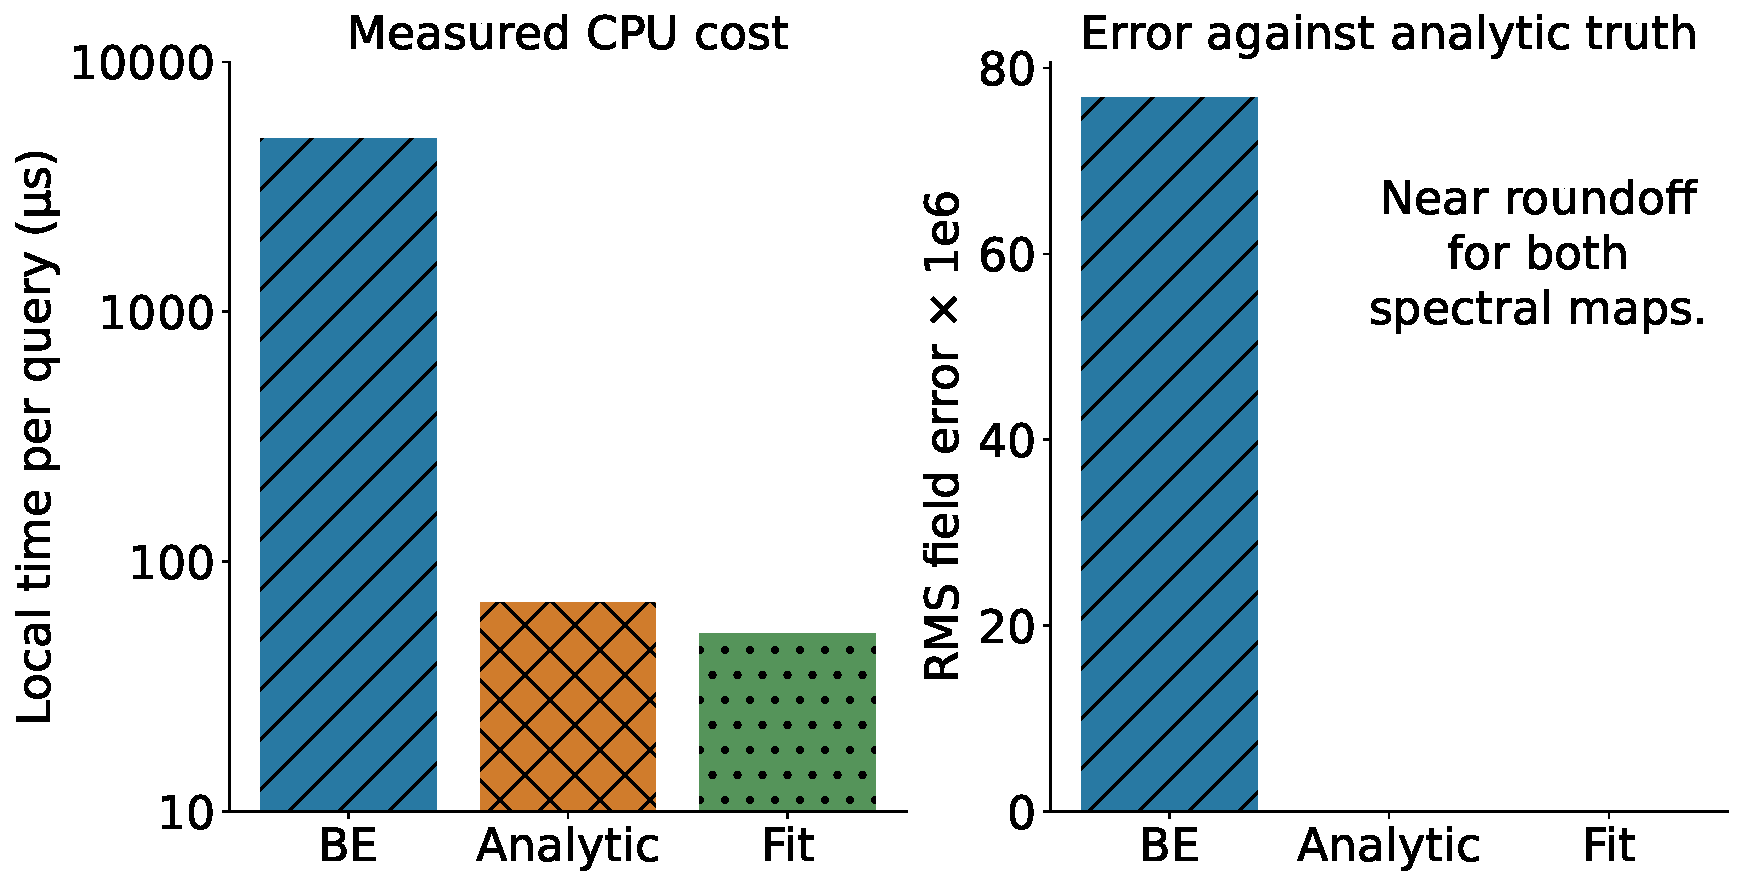
\includegraphics[width=.96\linewidth,height=.57\textheight,keepaspectratio]{cost-error.pdf}\par\smallskip
{\small Original local CPU timing and analytic-reference error for one synthetic heat case. Medians use seven batches of ten warm queries. Setup is recorded separately; these timings are not portable or paper performance results.}
\end{minipage}\end{center}
\section{A generator fitted through an Euler update}
\hypertarget{note-a-generator-fitted-through-an-euler-update}{}\label{note:a-generator-fitted-through-an-euler-update}
{\small \href{slides.html\#frame=the-exact-scalar-flow\&step=1}{Slides for this section}}\par
Consider the scalar decay equation y\ensuremath{^{\prime}}=\ensuremath{-}2 y, whose exact one-step multiplier at a training step of 0.1 is exp(\ensuremath{-}0.2). Suppose we fit a constant generator a through a forward-Euler update y\_new=y\_old+0.1 a y\_old. Matching the observed multiplier gives a=[exp(\ensuremath{-}0.2)\ensuremath{-}1]/0.1, approximately\ensuremath{-}1.812692. This is not the true continuous rate\ensuremath{-}2. It is the rate that makes one particular discrete update match the sampled data.

Repeated Euler steps of the training size reproduce the exact sampled decay for this example. If we halve the inference step while keeping the fitted generator, however, we approach the continuous flow generated by\ensuremath{-}1.812692. That flow is biased relative to exp(\ensuremath{-}2 t). At time 0.5 the true value is about 0.367879, while the exact learned continuous flow is about 0.403998. Smaller numerical steps more accurately solve the learned equation, but that equation is not the true one.

This is an analytically transparent mechanism, not a reproduction of GFuNK's experiments. The verified paper reports inference-step and integration-scheme sensitivity and cautions that accuracy can depend on matching training discretization. A higher-order solver is not automatically a correction for a model fitted through a lower-order rollout. Model error, training discretization and inference error must be examined together.

\[
a_{\Delta}=\frac{e^{-\lambda\Delta}-1}{\Delta},\quad(1+\Delta a_\Delta)y=e^{-\lambda\Delta}y
\]
Matching a sampled update does not imply a\_Delta=\ensuremath{-}lambda. The limit as training Delta\ensuremath{\to}0 is the true rate.

Matching an Euler step to exact scalar data requires
\[
 1+\Delta a_\Delta=e^{-\lambda\Delta},\qquad
 a_\Delta=-\lambda+\frac{\lambda^2}{2}\Delta+O(\Delta^2).
\]
The fitted generator is less negative than the true rate for $\lambda,\Delta>0$. At the training step, repeated Euler updates match the exact sampled multiplier; this cancellation is specific to that step and fitting construction.
\begin{center}\begin{minipage}{.98\linewidth}\centering
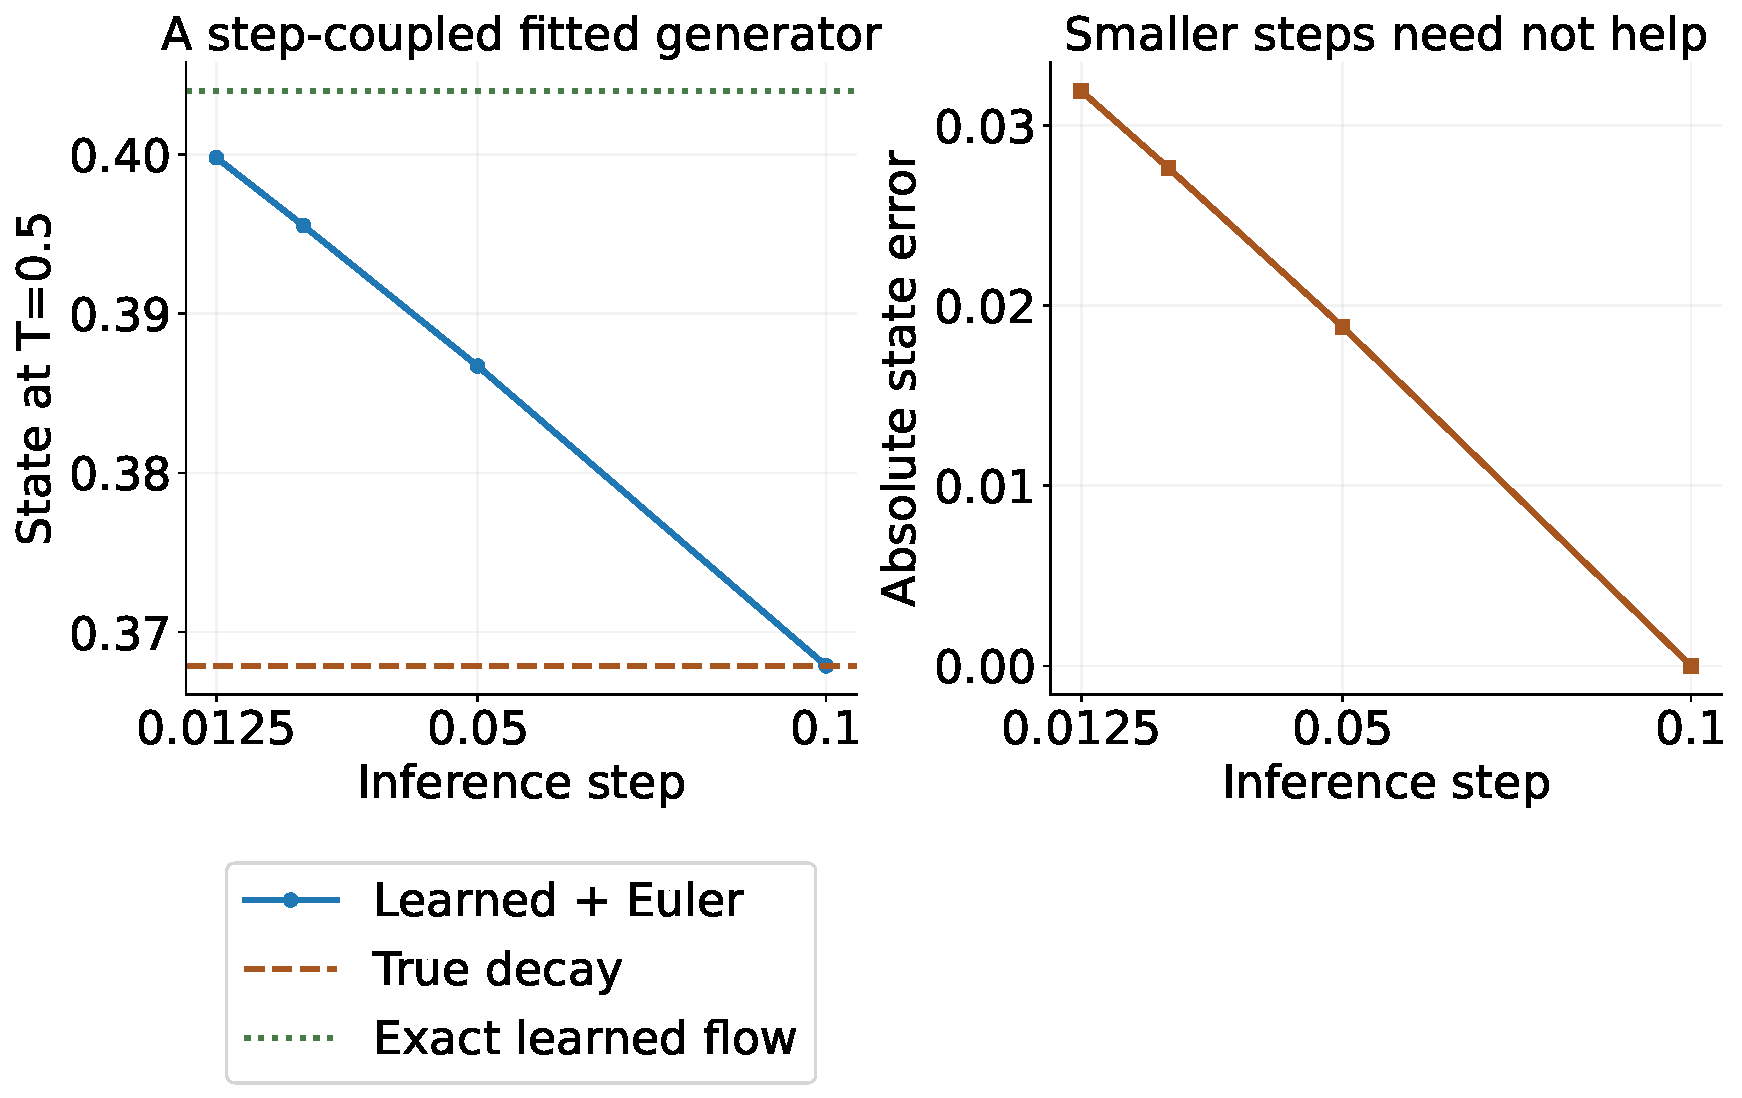
\includegraphics[width=.96\linewidth,height=.57\textheight,keepaspectratio]{learned-step.pdf}\par\smallskip
{\small Original scalar decay counterexample. Euler at the training step matches sampled truth; smaller steps approach a biased learned continuous flow. No GFuNK network is run.}
\end{minipage}\end{center}
\section{Training resolution and inference resolution}
\hypertarget{note-training-resolution-and-inference-resolution}{}\label{note:training-resolution-and-inference-resolution}
{\small \href{slides.html\#frame=refine-inference-while-holding-the-fit-fixed-panel-1\&step=1}{Slides for this section}}\par
A comparison should include controlled perturbations tied to the claim. To test a new initial-condition family, keep the equation, grid and timing protocol fixed while changing the designated inputs. To test geometry transfer, hold out entire geometries rather than snapshots from those geometries. To test resolution transfer, resample the same continuous problem and distinguish representation error from changed physical assumptions. Record the split rule before inspecting the final test outcomes.

Use more than one appropriate observable. A field norm can expose amplitude or spatial errors that a correlation misses. A local arrival time may be scientifically relevant but can be undefined when activation never occurs. Conservation and admissibility checks detect some numerical defects but do not guarantee accurate timing or spatial structure. Include negative controls and known limiting cases, such as no stimulus, zero coupling or a constant diffusion field, when they bear on the equations being studied.

The reference itself needs a budget. Refine space and time where appropriate, compare with an independent solver or an analytic case when available, and report residual uncertainty. A surrogate trained on a biased reference may learn that bias faithfully. If a discrepancy appears only on a new regime, do not immediately label it a software bug: first determine whether the model contract, numerical approximation or data distribution changed.

At inference step $h=T/n$ with $a_\Delta$ fixed,
\[
 (1+ha_\Delta)^n\longrightarrow e^{Ta_\Delta}
 \quad\text{as }h\to0.
\]
The discrepancy from $e^{-\lambda T}$ survives this limit. With $y(0)=1$, $\lambda=2$, $\Delta=.1$ and $T=.5$, the two limits are approximately $.403998$ and $.367879$. Sending the training step $\Delta$ to zero is a different limit and recovers $a_\Delta\to-\lambda$.
\section{The domain of a computational replacement claim}
\hypertarget{note-the-domain-of-a-computational-replacement-claim}{}\label{note:the-domain-of-a-computational-replacement-claim}
{\small \href{slides.html\#frame=an-admissible-computational-replacement\&step=1}{Slides for this section}}\par


A computational replacement claim is conditional on an error tolerance, input regime, output horizon and query workload. A faster method outside the required tolerance is not an admissible replacement. Conversely, a narrow exact family can make a simple analytic comparator preferable to either a general solver or a trained model. The relevant comparison follows from the mathematical problem, not from a preferred architecture.
\bigskip
\section*{Exercises}
\par\noindent\begin{minipage}{\linewidth}
\subsection*{E1. Amortize the complete setup}
A hypothetical workflow has C0=\allowbreak{}60 s, Cr=\allowbreak{}0.5 s and Cs=\allowbreak{}0.01 s. Assume both methods satisfy the required error.

\textbf{a} Find the first integer query count for which the surrogate is strictly cheaper.

\end{minipage}\par\medskip
\textbf{b} How does the conclusion change if Cs=\allowbreak{}0.6 s?

\par\noindent\begin{minipage}{\linewidth}
\subsection*{E2. Fit an update rather than a continuous rate}
True decay is y$^{\prime}$=\allowbreak{}-y with y(0)=\allowbreak{}1. A forward-Euler generator is fitted to exact pairs separated by training step 0.5.

\textbf{a} Derive the fitted generator and compare it with the true rate.

\end{minipage}\par\medskip
\textbf{b} Write the prediction at time 0.5 using two inference steps of 0.25. Explain why it differs from the true value.

\par\noindent\begin{minipage}{\linewidth}
\subsection*{E3. Separate error sources}
In one compatible absolute norm, surrogate-to-reference error is at most 0.01 and reference-to-equation error at most 0.02.

\textbf{a} Give a guaranteed upper bound for surrogate-to-equation error. Is equality required?

\end{minipage}\par\medskip
\textbf{b} Does this bound quantify error against experimental tissue data?

\par\noindent\begin{minipage}{\linewidth}
\subsection*{E4. Design a fair claim test}
A proposed claim is that a surrogate predicts unseen anatomies cheaply and accurately.

\textbf{a} Specify a split rule, accuracy observable and reference check that make the claim testable.

\end{minipage}\par\medskip
\textbf{b} Specify the timing boundary and one confounder to report.

\section*{References}
\noindent\begin{minipage}{\linewidth}
Zan Ahmad, Advanced Topics in Computational Cardiology syllabus, Fall 2024. PDF pages 1--2.

\end{minipage}\par\medskip
\noindent\begin{minipage}{\linewidth}
Loeffler, Ahmad, Chen and collaborators, Graph Fourier Neural Kernels: Learning Full PDE Trajectories Across Geometries and Anisotropic Parameter Fields. Main text section 3, pages 12--13; methods pages 14--18; SI sectionS 7, SI 13--14 / PDF 34--35.

\end{minipage}\par\medskip
\end{document}
